\documentclass{beamer}
\usepackage{pgfpages}
\usepackage[backend=bibtex]{biblatex}
\usepackage{multicol}
\usepackage{multimedia}
\usepackage[absolute,overlay]{textpos}
\usepackage{parskip}
\usepackage{hyperref}
\usepackage{lmodern}
\usepackage{bbding}
\usepackage[absolute,overlay]{textpos}
\usepackage{framed} %Used to shade important equations, color devined with shadecolor
\hypersetup{colorlinks=true, urlcolor=blue}
\setlength{\parskip}{\smallskipamount}
\colorlet{shadecolor}{cyan}
%\usepackage[texcoord,grid,gridunit=mm,gridcolor=red!10,subgridcolor=green!10]{eso-pic} %DELETE when done with grid
\setbeameroption{hide notes} % Only slides
%\setbeameroption{show only notes} % Only notes
%\setbeameroption{show notes on second screen=right} % Both
%\bibliography{../../papers/references.bib}
\setbeamerfont{footnote}{size=\tiny}
%\AtEveryCitekey{\clearfield{title}}

%
% Choose how your presentation looks.
%
% For more themes, color themes and font themes, see:
% http://deic.uab.es/~iblanes/beamer_gallery/index_by_theme.html
%
\mode<presentation>
{
\usetheme{Warsaw}      % or try Darmstadt, Madrid, Warsaw, ...
\usecolortheme{default} % or try albatross, beaver, crane, ...
\usefonttheme{default}  % or try serif, structurebold, ...
\setbeamertemplate{navigation symbols}{}
\setbeamertemplate{caption}[numbered]
} 

\usepackage[english]{babel}
%\usepackage[utf8x]{inputenc} %Doesn't play well with biblatex
\usepackage{amssymb}
\usepackage{bm}
\usepackage{color}
\usepackage{graphicx}
\setbeamercovered{invisible}
\setbeamercovered{%
again covered={\opaqueness<1->{100}}} %This changes the opaqueness of each bullet

\newcommand{\red}[1]{{\color{red}{#1}}}
\newcommand{\checkH}[2]{\begin{textblock*}{1cm}(#1,#2){\Huge \red{\Checkmark}}\end{textblock*}}
\newcommand{\checkh}[2]{\begin{textblock*}{1cm}(#1,#2){\huge \red{\Checkmark}}\end{textblock*}}
\newcommand{\checkL}[2]{\begin{textblock*}{1cm}(#1,#2){\Large \red{\Checkmark}}\end{textblock*}}
\newcommand{\checkl}[2]{\begin{textblock*}{1cm}(#1,#2){\large \red{\Checkmark}}\end{textblock*}}
\renewcommand{\rm}[1]{\mathrm{#1}}

\title[{\color{white}{Chapters 4.1-3}}]{Physics 121: \\ 2D Motion, Projectiles, Relative Motion}
\author{Cody Petrie}
\institute{Mesa Community College}
\date{}

\begin{document}

%\setbeamertemplate{frametitle}[default][center]
\begin{frame}
\titlepage
\end{frame}

% Uncomment these lines for an automatically generated outline.
%\begin{frame}{Outline}
%  \tableofcontents
%\end{frame}

% Commands to include a figure:
%\begin{figure}
%\includegraphics[width=\textwidth]{your-figure's-file-name}
%\caption{\label{fig:your-figure}Caption goes here.}
%\end{figure}

\begin{frame}{Reminders}
\begin{itemize}
   \item The first exam is this coming Tuesday (19 Sep).
   \item Does anybody not have a book yet?
   \item Today we are going to apply the vector stuff we learned to motion!
\end{itemize}
\end{frame}

\begin{frame}{2D Motion}
\begin{center}
   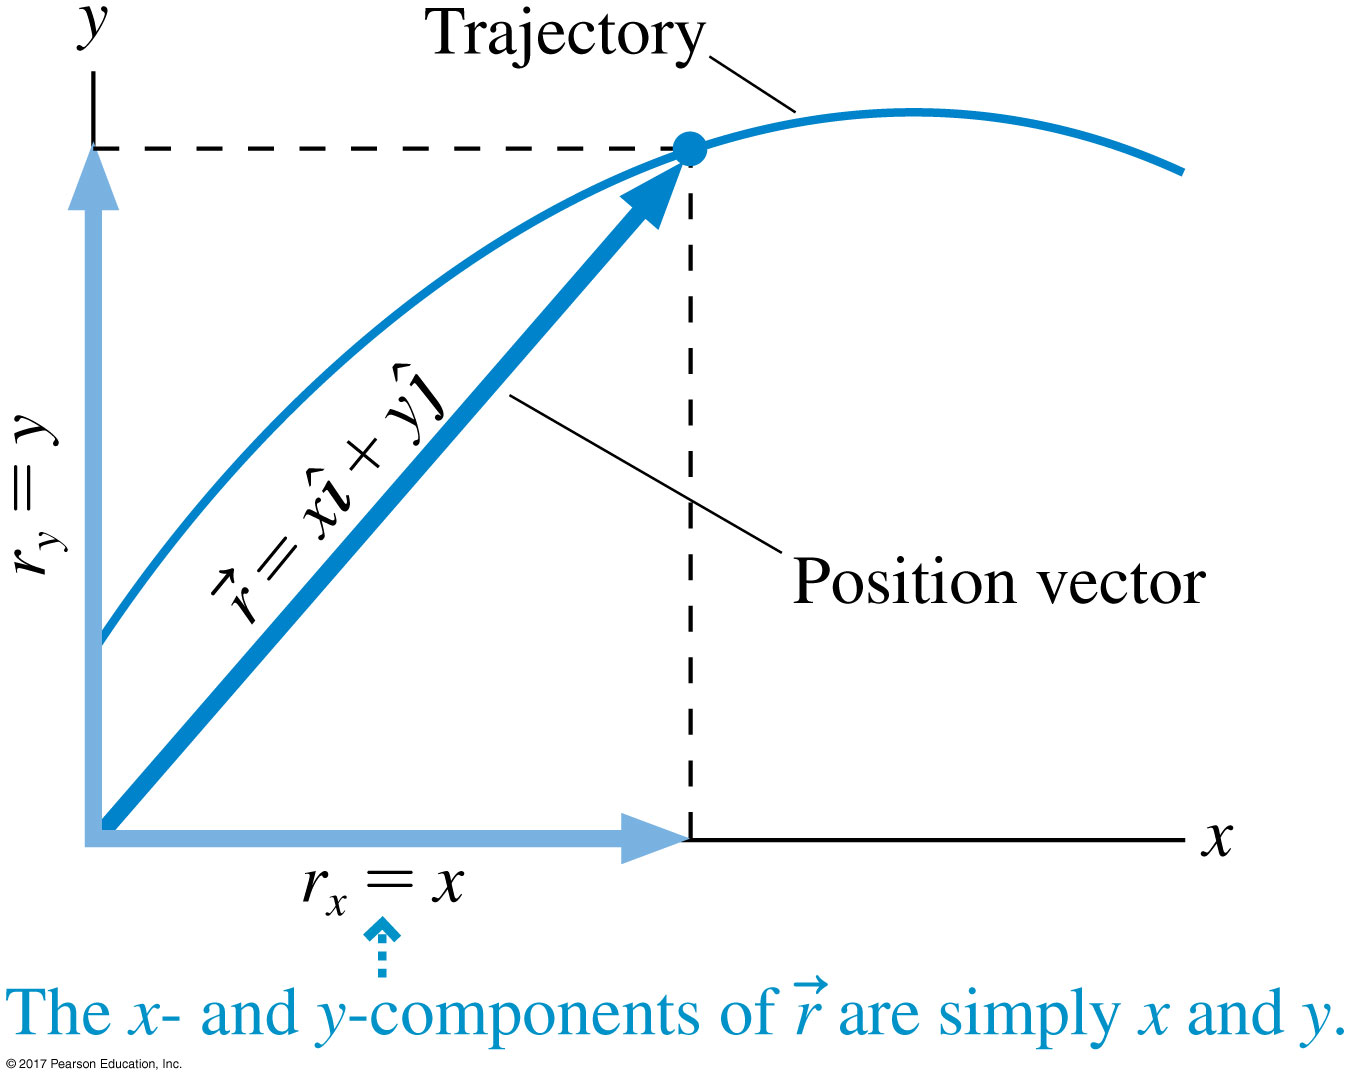
\includegraphics[width=0.5\textwidth]{../figures/04_01_Figure.jpg}
\end{center}
\begin{itemize}
   \item This is the trajector of a particle in the xy-plane. This is a ``picture" of the motion.
   \item Notice that any at any time the motion can be described by a position vector $\vec{r}$, just like we talked about last week.
\end{itemize}
\end{frame}

\begin{frame}{2D Motion}
\begin{center}
   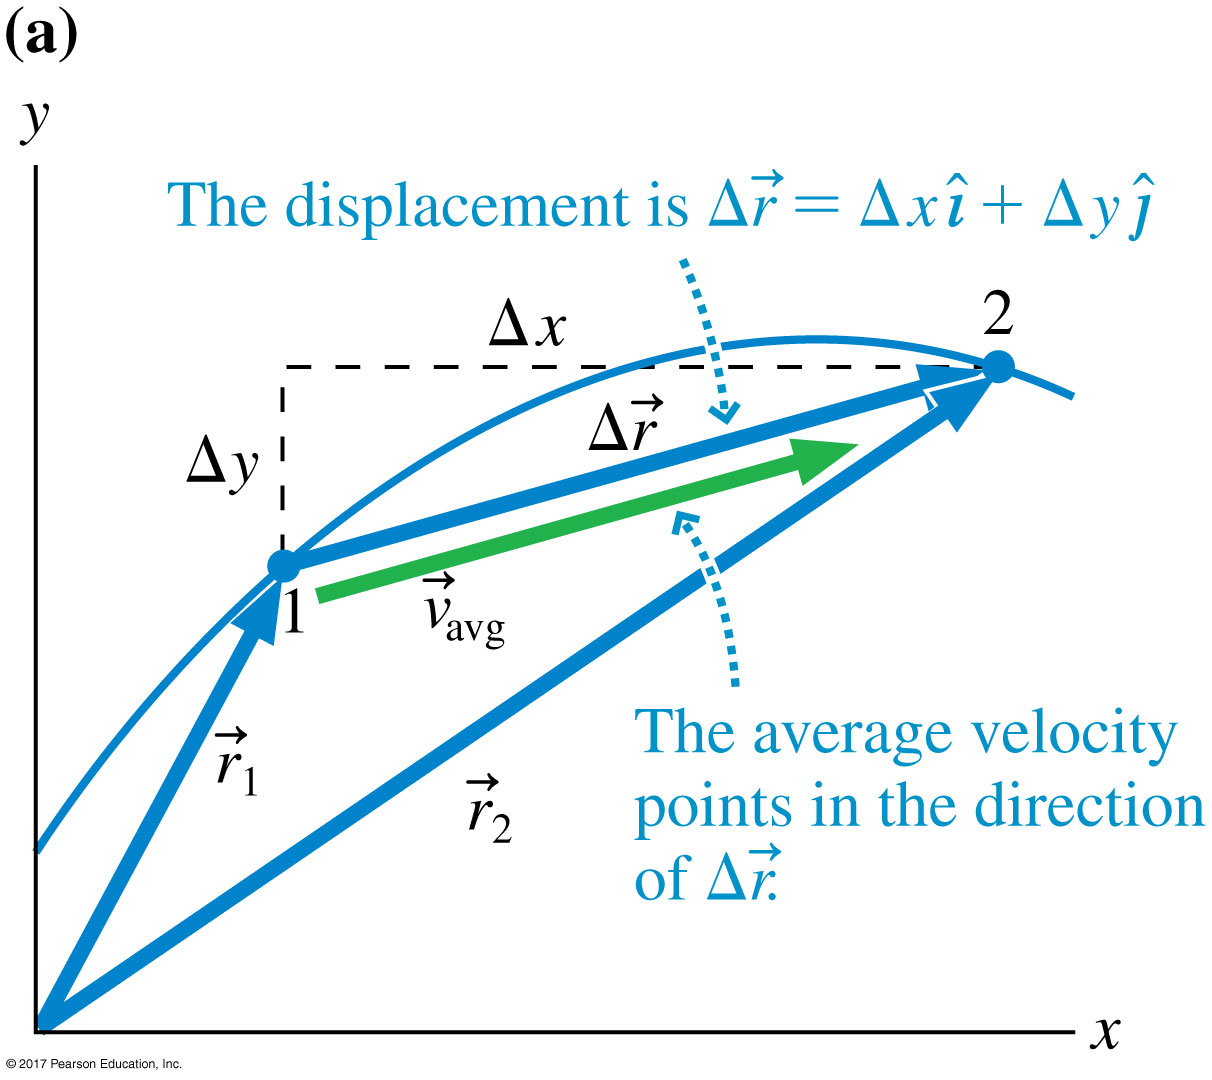
\includegraphics[width=0.5\textwidth]{../figures/04_02_FigureA.jpg}
\end{center}
\begin{itemize}
   \item This is the trajector of a particle going from position $\vec{r}_1$ to position $\vec{r}_2$.
   \item Notice that the average velocity points in the direction of the displacement vector
   \begin{equation*}
      \vec{v}_{ave} = \frac{\Delta \vec{r}}{\Delta t} = \frac{\Delta x}{\Delta t}\hat{i} + \frac{\Delta y}{\Delta t}\hat{j}
   \end{equation*}
\end{itemize}
\end{frame}

\begin{frame}{2D Motion}
\begin{center}
   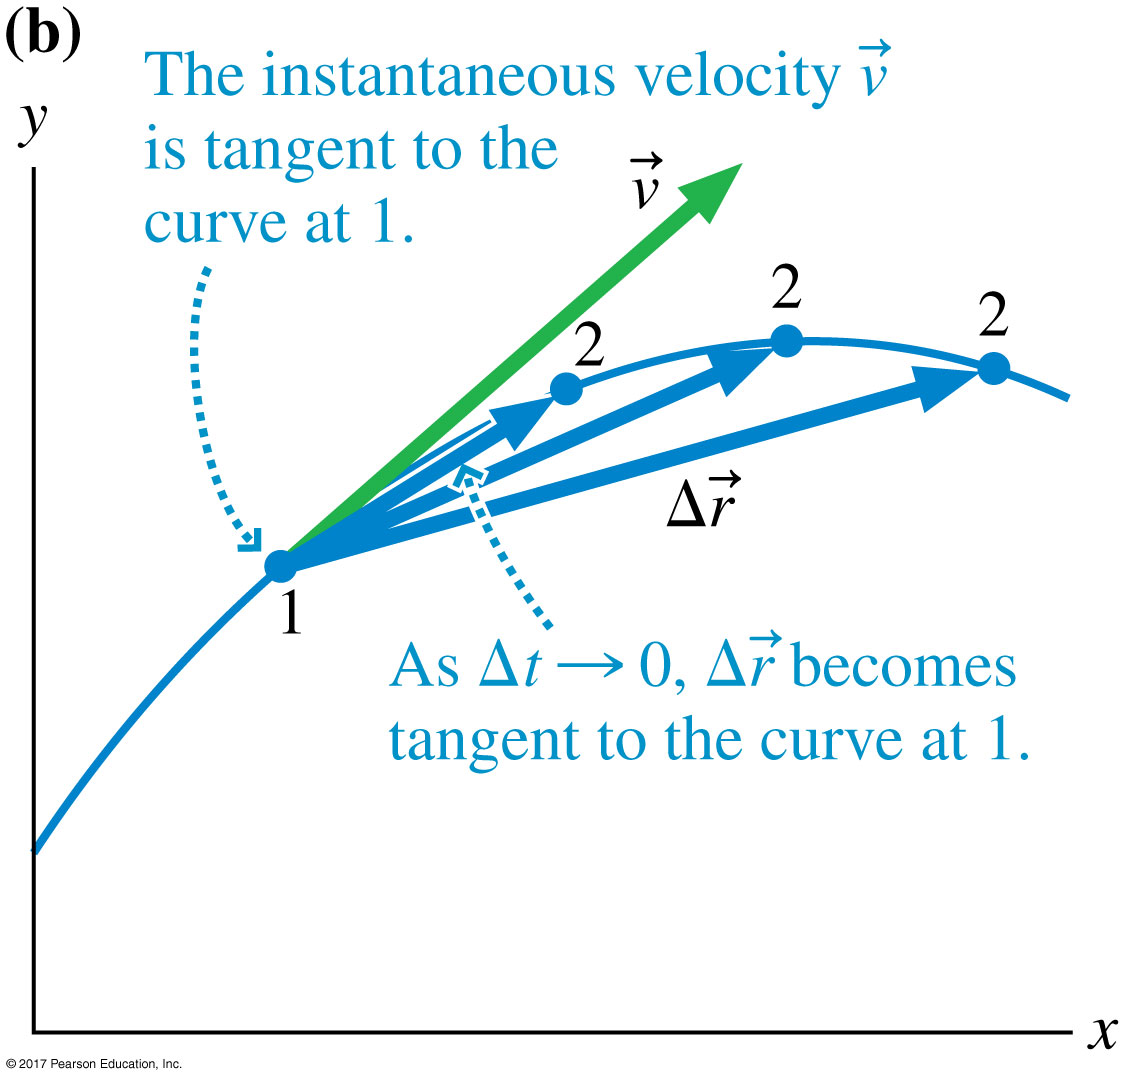
\includegraphics[width=0.5\textwidth]{../figures/04_02_FigureB.jpg}
\end{center}
\begin{itemize}
   \only<1>{
      \item The average velocity approaches the instantaneous velocity as the spacing decreases, which you can see above.
      \item The instantaneous velocity is the limit (derivative)
      \begin{equation*}
         \vec{v} = \lim\limits_{\Delta t \rightarrow 0} \frac{\Delta \vec{r}}{\Delta t} = \frac{d\vec{r}}{dt} = \frac{dx}{dt}\hat{i} + \frac{dy}{dt}\hat{j}
      \end{equation*}
   }
   \only<2>{
      \item The instantaneous velocity can also be written as
      \begin{equation*}
         \vec{v} = v_x\hat{i} + v_y\hat{j}
      \end{equation*}
      where
      \begin{equation*}
         v_x = \frac{dx}{dt}~~~~\text{and}~~~~ v_y = \frac{dy}{dt}
      \end{equation*}
   }
\end{itemize}
\end{frame}

\begin{frame}{Quick Check}
\begin{center}
   What is the instantaneous velocity at time $t$ of the object that follows the trajectory $\vec{r}(t) = (4+2t^2-t^3)\hat{i} - (3\pi t^5)\hat{j}$? \\~\\ \uncover<2>{$\vec{v}(t) = \frac{d\vec{r}}{dt} = (4t-3t^2)\hat{i} - (15\pi t^4)\hat{j}$}
\end{center}
\end{frame}

\begin{frame}{2D Motion}
\begin{center}
   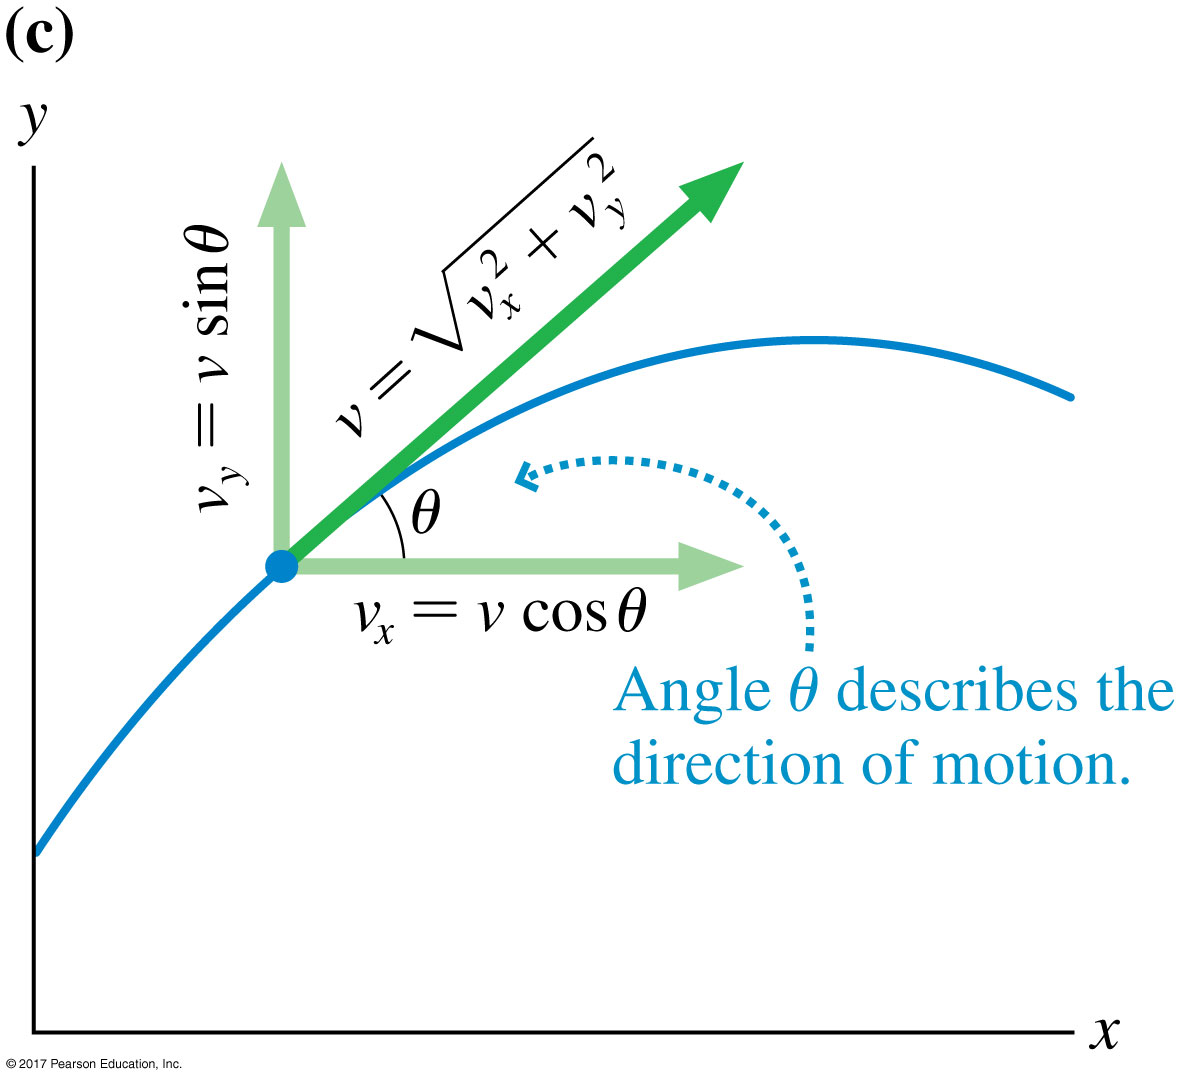
\includegraphics[width=0.5\textwidth]{../figures/04_02_FigureC.jpg}
\end{center}
\begin{itemize}
   \item If we know the angle of the motion with respect to the positive x-axis we can calculate the components and speed.
   \item Conversely, if we know the components we can determine the direction of motion with
   \begin{equation*}
      \theta = \tan^{-1}\left(\frac{v_y}{v_x}\right)
   \end{equation*}
\end{itemize}
\end{frame}

\begin{frame}{Quick Check}
\begin{center}
   During which time interval or intervals is the particle described by these position graphs at rest? More than one may be correct
   \begin{columns}
   \begin{column}{0.15\textwidth}
   \begin{enumerate}[a.]
      \item 0-1 s
      \item 1-2 s
      \item 2-3 s
      \item 3-4 s
   \end{enumerate}
   \end{column}
   \begin{column}{0.85\textwidth}
      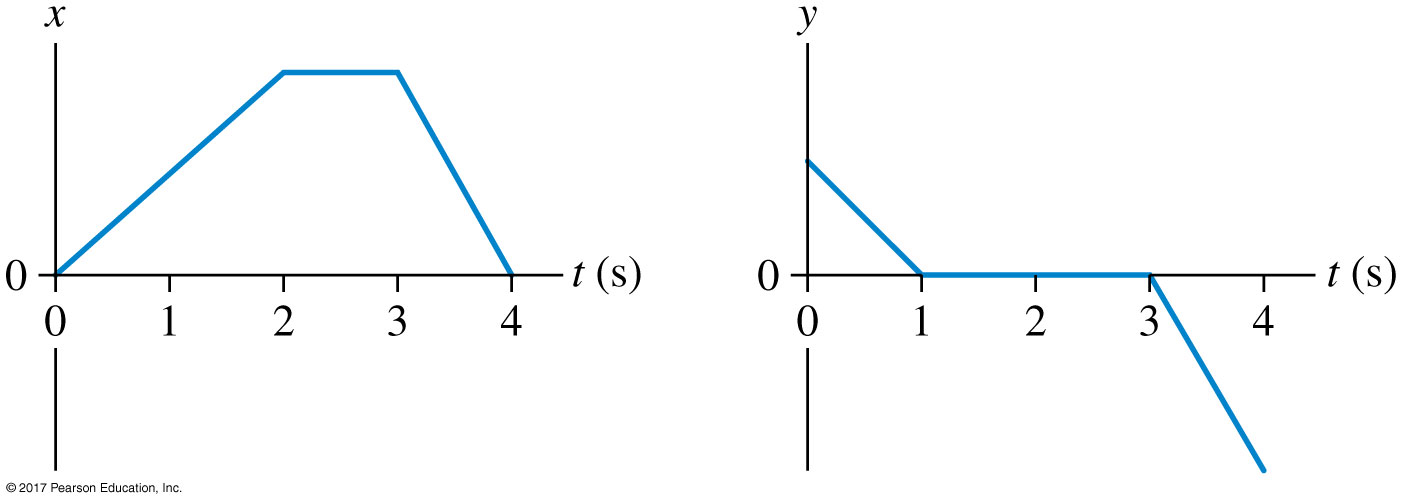
\includegraphics[width=\textwidth]{../figures/Figure_STT4_1.jpg}
   \end{column}
   \end{columns}
\end{center}
\only<2>{\checkl{0.3cm}{5.2cm}}
\end{frame}

\begin{frame}{2D Acceleration}
\begin{itemize}
   \item The average acceleration is defined just like it was before in 1D, but now we need to take 2 dimensions into account
   \begin{equation*}
      \vec{a}_{ave} = \frac{\Delta \vec{v}}{\Delta t}
   \end{equation*}
   \item<2-> Here is an example of a 2D acceleration graphically.
   \begin{center}
      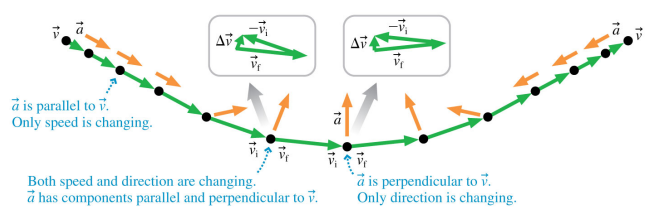
\includegraphics[width=\textwidth]{../figures/EX04_02.png}
   \end{center}
\end{itemize}
\end{frame}

\begin{frame}{2D Acceleration}
\begin{center}
   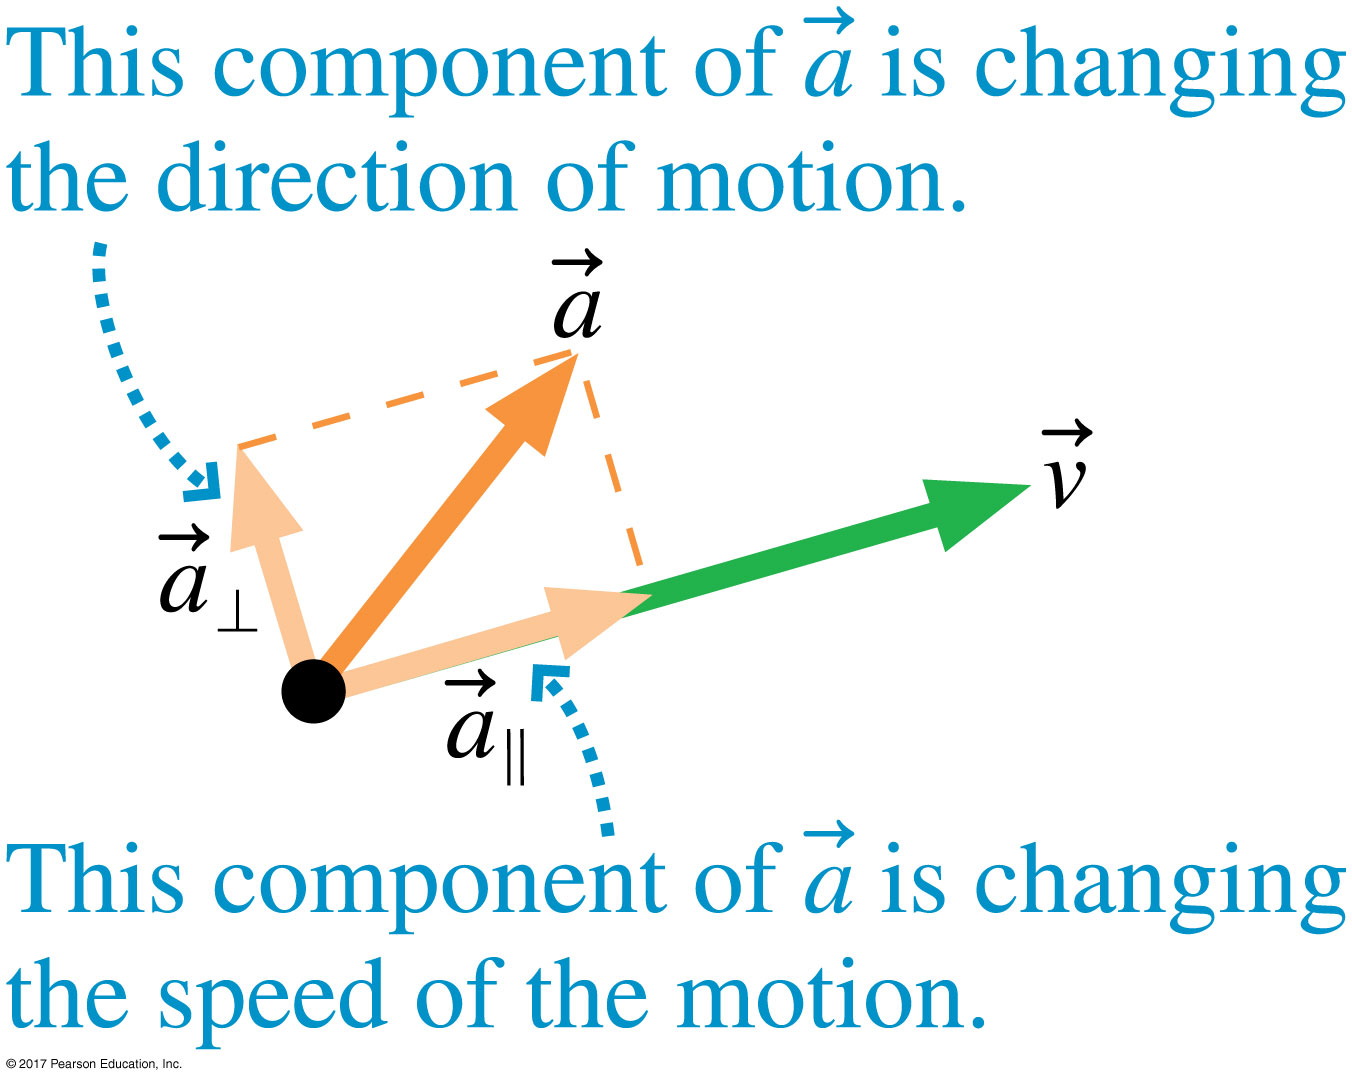
\includegraphics[width=0.5\textwidth]{../figures/04_05_Figure.jpg}
\end{center}
\begin{itemize}
   \item<1-> There are two parts to acceleration, one parallel to the velocity $\vec{a}_\perp$, and one parallel to the velocity, $\vec{a}_\parallel$.
   \item<1-> Which one causes an object to change speed?
   \begin{itemize}
      \item<2-> $\vec{a}_\parallel$
   \end{itemize}
   \item<3-> Which one causes an object to change direction?
   \begin{itemize}
      \item<4-> $\vec{a}_\perp$
   \end{itemize}
\end{itemize}
\end{frame}

\begin{frame}{2D Acceleration}
\begin{center}
   You can maybe see this better in this figure
   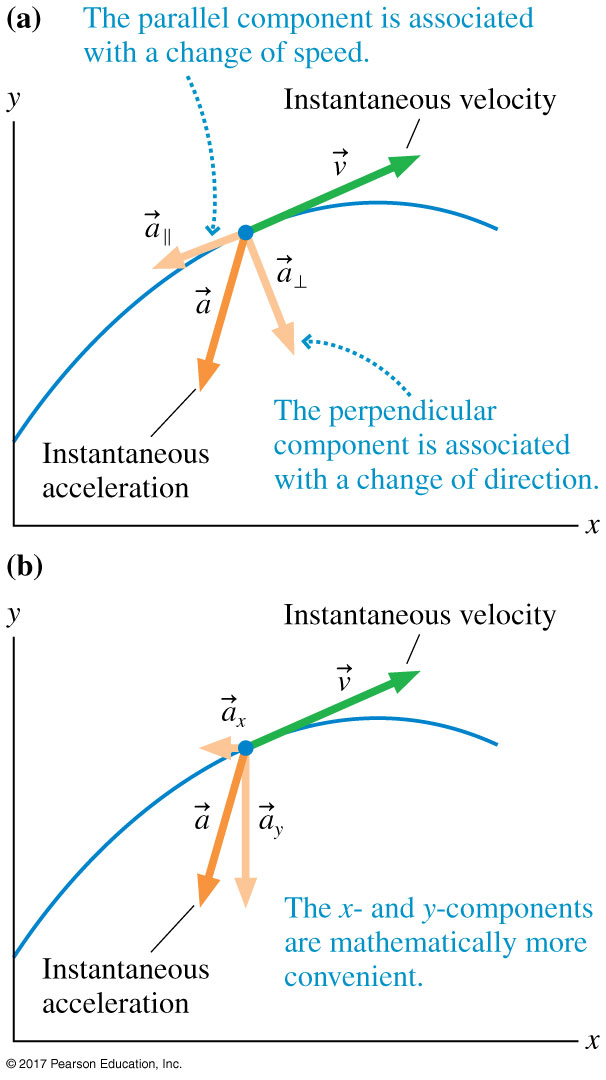
\includegraphics[width=0.4\textwidth]{../figures/04_06_Figure.jpg}
\end{center}
\end{frame}

\begin{frame}{2D Accleration}
\begin{itemize}
   \item The x- and y-components look the same as they did for velocity.
   \begin{equation*}
      \vec{a} = a_x\hat{i} + a_y\hat{j} = \frac{d\vec{v}}{dt} = \frac{dv_x}{dt}\hat{i} + \frac{dv_y}{dt}\hat{j}
   \end{equation*}
   where
   \begin{equation*}
      a_x = \frac{dv_x}{dt}~~~~\text{and}~~~~ a_y = \frac{dv_y}{dt}
   \end{equation*}
\end{itemize}
\end{frame}

\begin{frame}{2D CONSTANT Acceleration}
\begin{itemize}
   \item When we had constant acceleration in 1D motion what equations did we use?
   \item<2-> They were called kinematic equations. In 2D you just have two sets, one for each dimension.
   \begin{columns}
   \begin{column}{0.5\textwidth}
   \begin{align*}
      x_f &= x_i + v_{ix}t + \frac{1}{2}a_xt^2 \\
      v_{fx} &= v_{ix} + a_xt \\
      v_{fx}^2 &= v_{ix}^2 + 2a_x\Delta x
   \end{align*}
   \end{column}
   \begin{column}{0.5\textwidth}
   \begin{align*}
      y_f &= y_i + v_{iy}t + \frac{1}{2}a_yt^2 \\
      v_{fy} &= v_{iy} + a_yt \\
      v_{fy}^2 &= v_{iy}^2 + 2a_y\Delta y
   \end{align*}
   \end{column}
   \end{columns}
   \item<3-> You have to keep track of MANY variables in 2D problems. Make sure to be more careful when setting up problems.
\end{itemize}
\end{frame}

\begin{frame}{Quick Check}
\begin{center}
   This acceleration will cause the particle to
   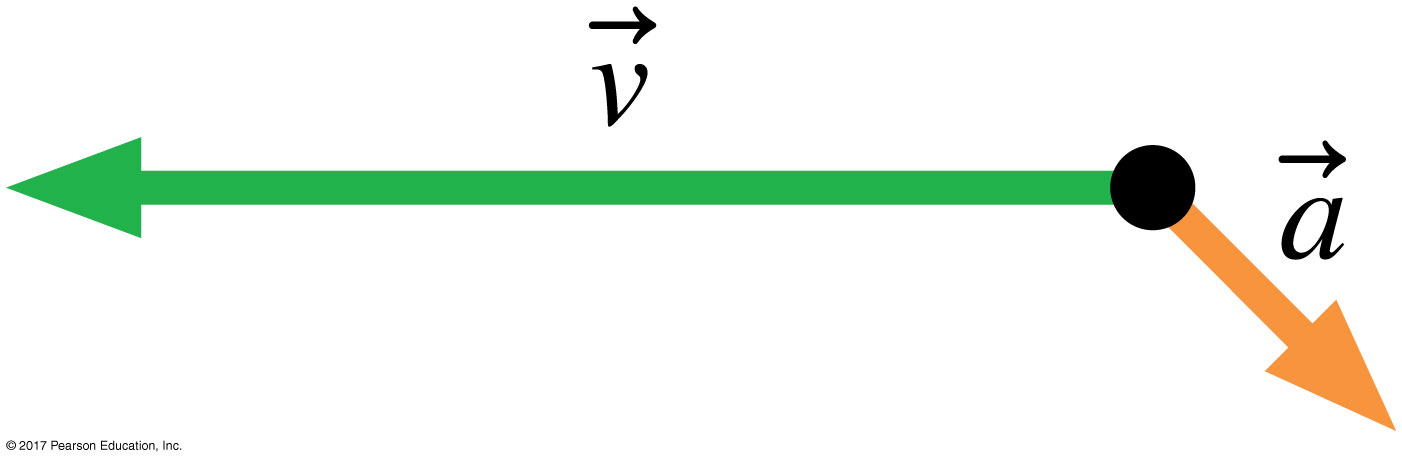
\includegraphics[width=0.7\textwidth]{../figures/Figure_STT4_2.jpg}
   \begin{enumerate}[a.]
      \item Speed up and curve upward
      \item Slow down and curve upward
      \item Move to the right and down
      \item Speed up and curve downward
      \item Slow down and curve downward
      \item Reverse direction
   \end{enumerate}
\end{center}
\only<2>{\checkl{0.6cm}{7.1cm}}
\end{frame}

\begin{frame}{Quick Check}
\begin{center}
   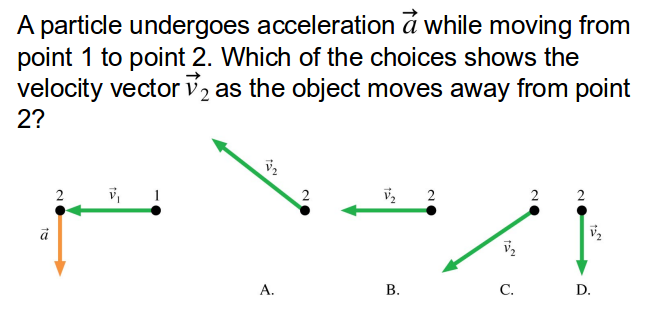
\includegraphics[width=\textwidth]{../figures/QC4_1.png}
\end{center}
\only<2>{\checkh{9.0cm}{6.8cm}}
\end{frame}

\begin{frame}{Projectile Motion}
\begin{center}
   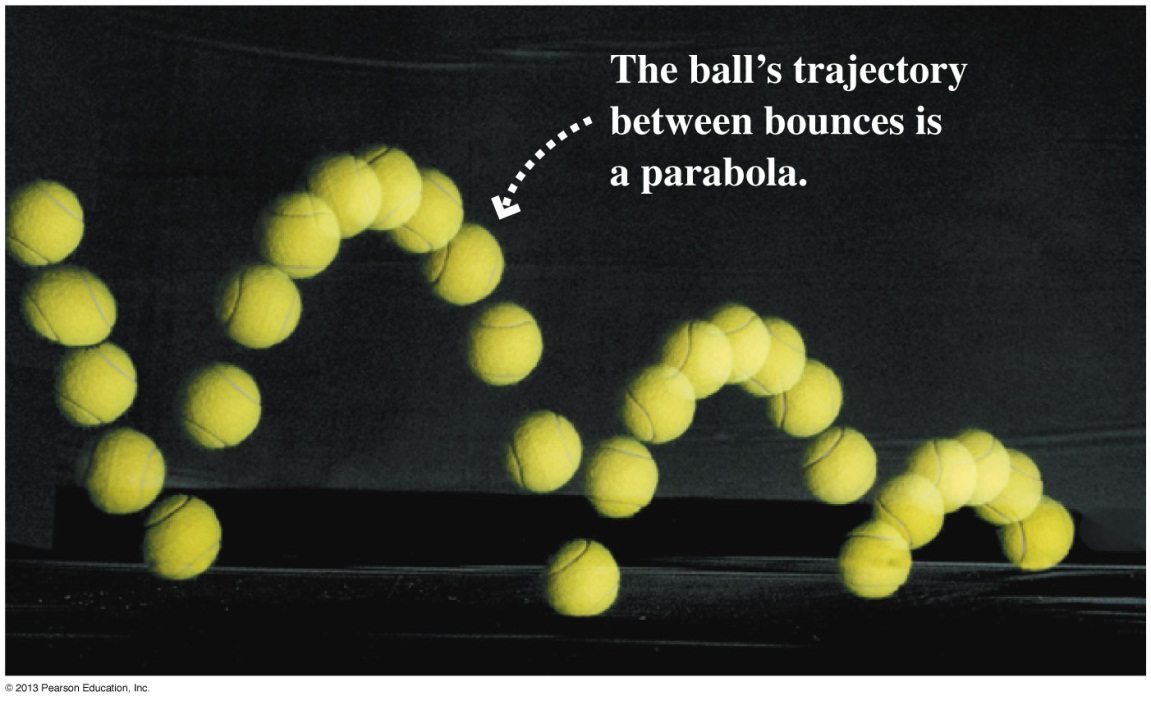
\includegraphics[width=0.5\textwidth]{../figures/parabola.jpg}
\end{center}
\begin{itemize}
   \item Projectile Motion is 2D motion where an object is only influenced by gravity. It's like 2D free fall motion.
\end{itemize}
\end{frame}

\begin{frame}{Projectile Motion}
\begin{center}
   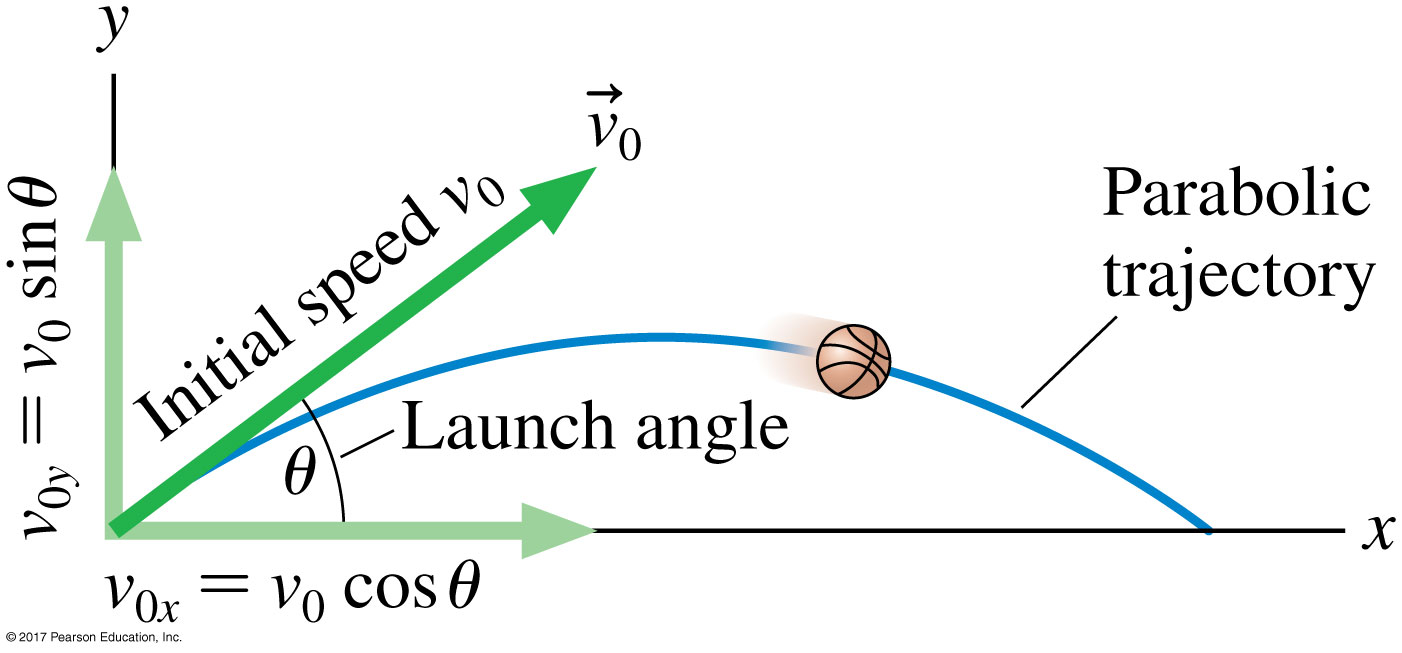
\includegraphics[width=0.5\textwidth]{../figures/projectile.jpg}
\end{center}
\begin{itemize}
   \item You can solve for the x and y components of the initial velocity, $v_{0x}$ and $v_{0y}$, given the angle, $\theta$.
   \item<2-> What are the objects horizontal and vertical accelerations?
   \begin{itemize}
      \item<3-> $a_x = 0$ m/s$^2$ and $a_y = -9.80$ m/s$^2$
   \end{itemize}
   \item<3-> Notice that just like with free fall $a_y=-g$.
\end{itemize}
\end{frame}

\begin{frame}{Projectile Motion}
\begin{itemize}
   \item If I have an objects that is launched at $t=0$ s and has the initial velocity $\vec{v}_0 = (9.8\hat{i} + 19.6\hat{j})$ m/s. What is the velocity at $t=1$ s and $t=2$ s?
\end{itemize}
\uncover<2>{
\begin{columns}
\begin{column}{0.5\textwidth}
\begin{center}
   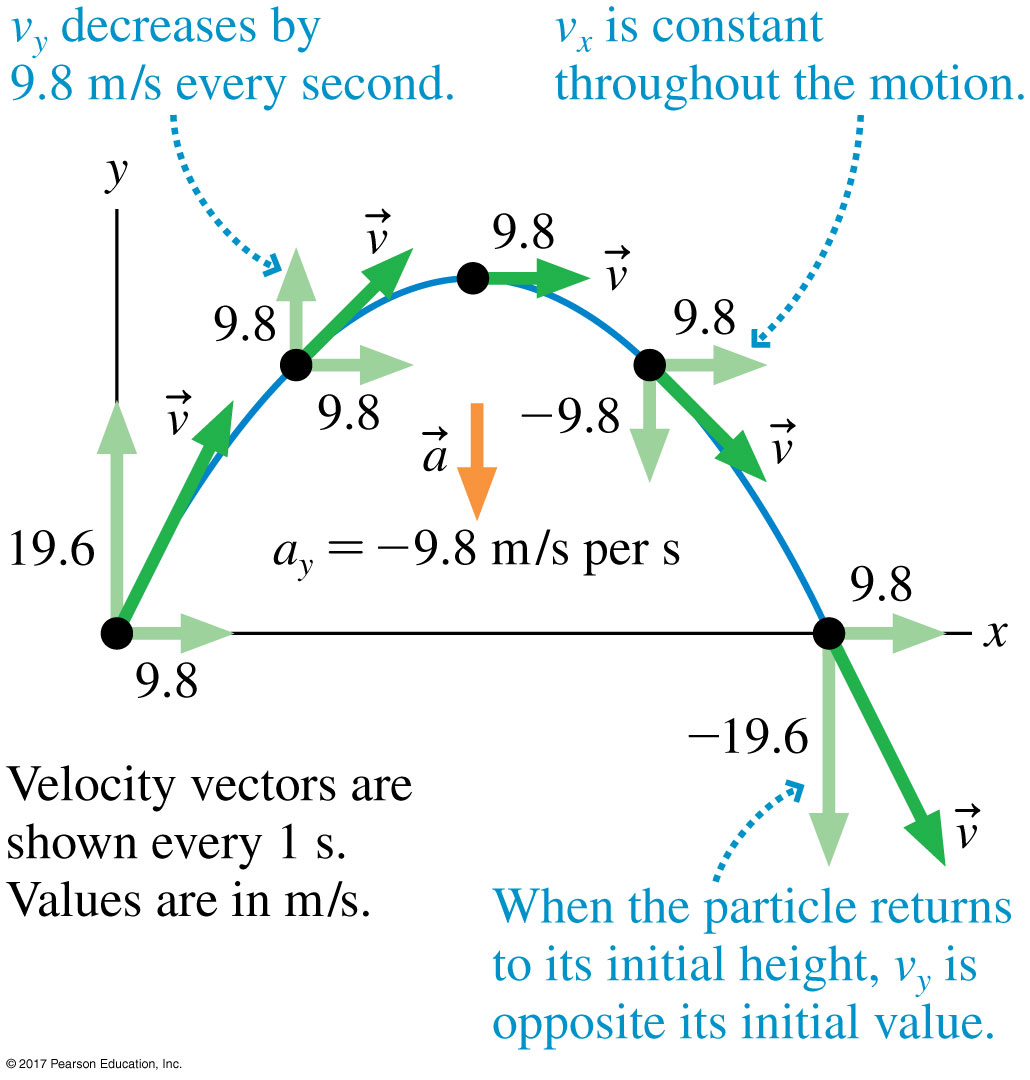
\includegraphics[width=\textwidth]{../figures/powerpoint4_3.jpg}
\end{center}
\end{column}
\begin{column}{0.5\textwidth}
\begin{itemize}
   \item $v_x$ never changes because there is no horizontal acceleration.
   \item $v_y$ decreases by 9.8 m/s every second.
\end{itemize}
\end{column}
\end{columns}
}
\end{frame}

\begin{frame}{Quick Check}
\begin{center}
   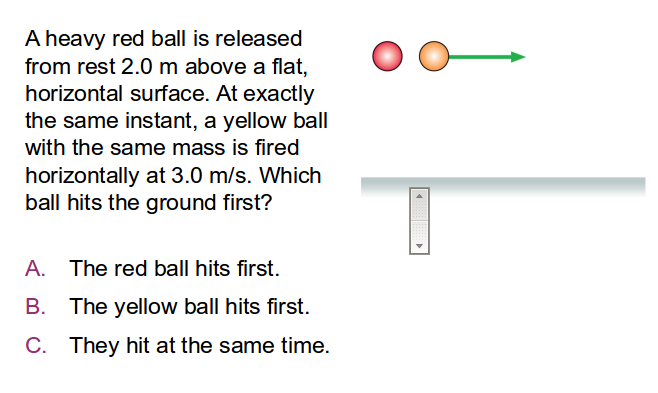
\includegraphics[width=\textwidth]{../figures/QC4_2.png}
\end{center}
\only<2>{\checkh{1.0cm}{6.6cm}}
\end{frame}

\begin{frame}{Quick Check}
\begin{center}
   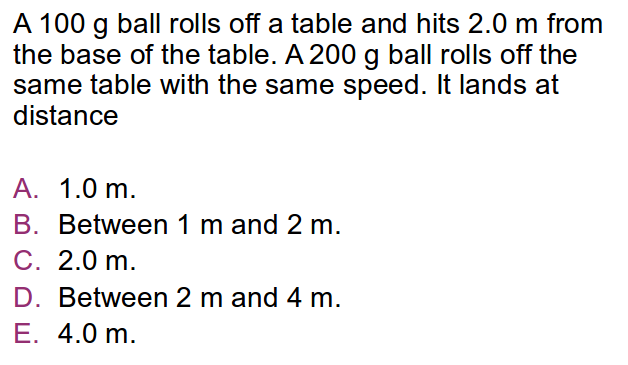
\includegraphics[width=\textwidth]{../figures/QC4_3.png}
\end{center}
\only<2>{\checkh{0.8cm}{5.6cm}}
\end{frame}

\begin{frame}{Quick Check}
\begin{center}
   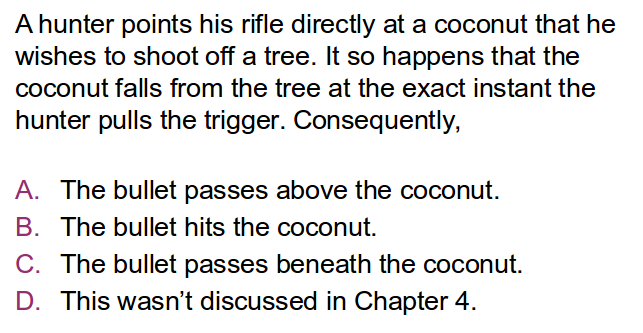
\includegraphics[width=\textwidth]{../figures/RQ4_2.png}
\end{center}
\only<2>{\checkh{0.7cm}{5.3cm}}
\end{frame}

\begin{frame}{Quick Check}
\begin{center}
   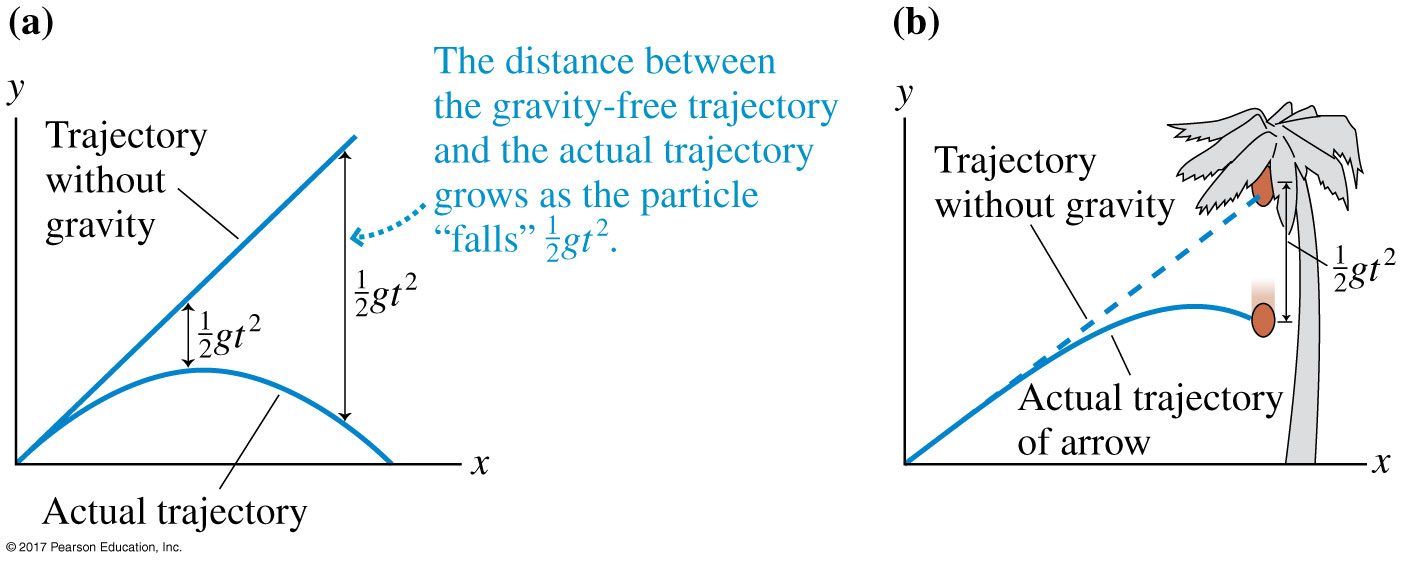
\includegraphics[width=\textwidth]{../figures/04_14_Figure.jpg}
\end{center}
\end{frame}

\begin{frame}{Projectile Range}
\begin{itemize}
   \item A projectile with initial speed $v_0$ has a launch angle of $\theta$ above the horizontal. How far does it travel over level ground before it returns to the same elevation from which it was launched?
   \begin{center}
   \uncover<2>{
   Begin with the equations
   \begin{align*}
      x_f &= x_i+v_{ix}t+1/2a_xt^2 \\
      y_f &= y_i+v_{iy}t+1/2a_yt^2
   \end{align*}
   }
   \uncover<3>{
   Notice that $x_i=a_x=y_f=y_i=0$, $a_y=-g$, $v_{ix}=v_0\cos(\theta)$ and $v_{iy}=v_0\sin(\theta)$ which leaves you with
   \begin{align*}
      x_f &= v_0\cos(\theta)t \\
      0 &= v_0\sin(\theta)t-1/2gt^2
   \end{align*}
   }
   \uncover<4>{
   Now solve for t in the y equation and plug it into the x equation, noticing and $\cos(\theta)\sin(\theta)=\sin(2\theta)$, which gives
   \begin{equation*}
      xf=\frac{2v_0^2}{g}\sin(2\theta) = \text{range}
   \end{equation*}
   }
   \end{center}
\end{itemize}
\end{frame}

\begin{frame}{Projectile Range}
\begin{center}
\begin{equation*}
   xf=\frac{2v_0^2}{g}\sin(2\theta) = \text{range}
\end{equation*}
Notice that the maximum of the range is then at 45$^\circ$.
\end{center}
\end{frame}

\begin{frame}{Relative Motion}
\begin{center}
   \color{blue}{\Huge Relative Motion}
\end{center}
\end{frame}

\begin{frame}{Relative Motion}
\begin{center}
   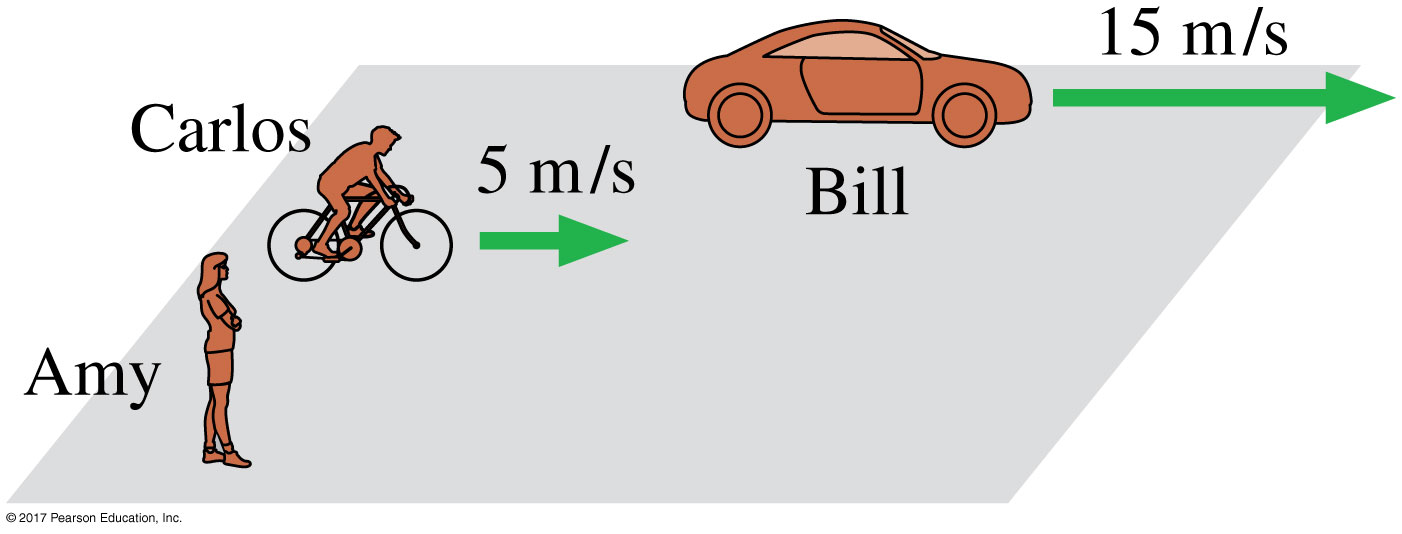
\includegraphics[width=0.7\textwidth]{../figures/04_17_Figure.jpg}
\end{center}
\begin{itemize}
   \item<1-> The figure below shows Amy and Bill watching Carlos on his bicycle. According to Amy, Carlos's velocity is $(v_x)_{CA} = +5$ m/s.
   \begin{itemize}
      \item<1-> The $CA$ subscript means ``C relative to A."
   \end{itemize}
   \item<2-> According to Bill, Carlos's velocity is $(v_x)_{CB} = -10$ m/s.
   \item<3-> Every velocity is measured relative to a certain observer. There is no ``true" velocity.
\end{itemize}
\end{frame}

\begin{frame}{Relative Motion}
\begin{itemize}
   \item The velocity of C relative to B is the velocity of C relative to A plus the velocity of A relative to B.
   \begin{center}
      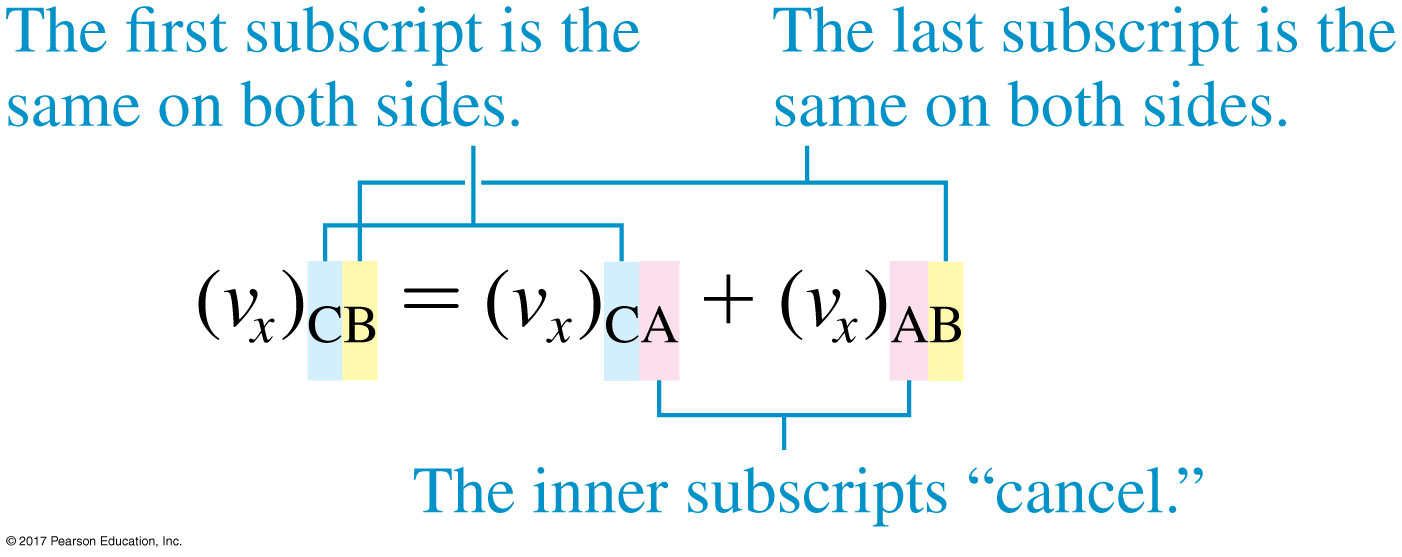
\includegraphics[width=0.7\textwidth]{../figures/EQ4_16.jpg}
   \end{center}
   \item If B is moving to the right relative to A, then A is moving to the left relative to B.
   \begin{equation*}
      (v_x)_{AB} = -(v_x)_{BA}
   \end{equation*}
\end{itemize}
\end{frame}

\begin{frame}{Relative Motion}
\begin{center}
   \Huge \href{https://www.youtube.com/watch?v=qQVDAMzo4mE}{Mythbusters - Relative Motion}
\end{center}
\end{frame}

\begin{frame}{Relative Motion}
\begin{itemize}
   \item The coordinate system that is used to make measurements is often called a {\bf reference frame}.
   \item<2-> In the figure, Object C is measured in two different reference frames, A and B.
\end{itemize}
\uncover<2>{
\begin{columns}
\begin{column}{0.6\textwidth}
\begin{center}
   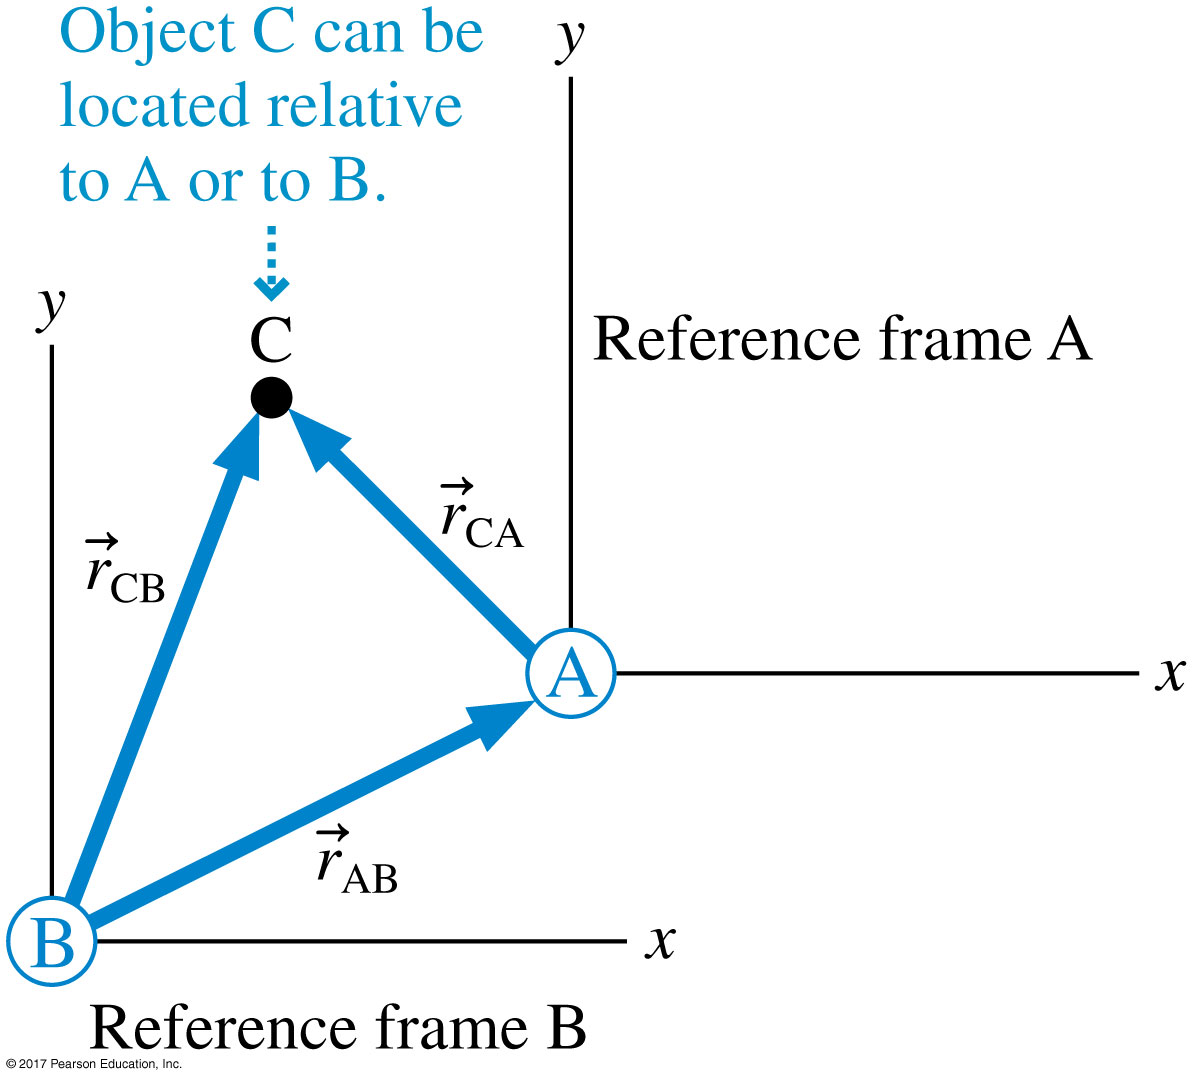
\includegraphics[width=\textwidth]{../figures/04_18_Figure.jpg}
\end{center}
\end{column}
\begin{column}{0.4\textwidth}
\begin{itemize}
   \item<3-> Notice here that $\vec{r}_{CB} = \vec{r}_{CA} + \vec{r}_{AB}$
   \item<4-> Also, since the relative velocities are just the derivatives of the relative positions we can say $\vec{v}_{CB} = \vec{v}_{CA} + \vec{v}_{AB}$. This is called a {\bf Galilean Transformation}.
\end{itemize}
\end{column}
\end{columns}}
\end{frame}

\begin{frame}{Quick Check}
\begin{center}
   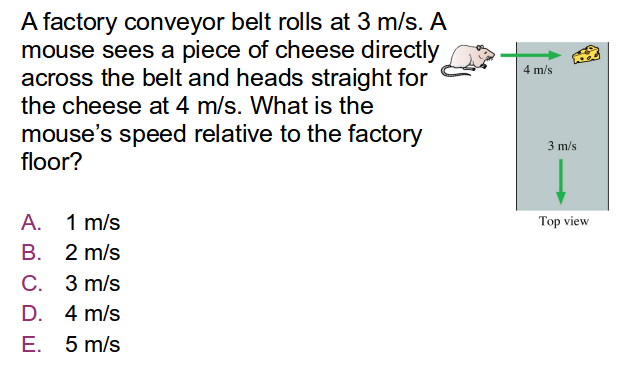
\includegraphics[width=\textwidth]{../figures/QC4_6.png}
\end{center}
\only<2>{
\checkl{1.1cm}{7.0cm}
   \begin{textblock*}{\textwidth}(4.3cm,5.4cm) % {block width} (coords)
      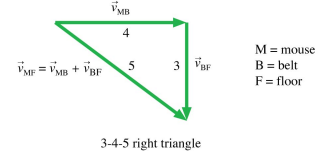
\includegraphics[width=6.0cm]{../figures/QC4_6-2.png}
   \end{textblock*}
}
\end{frame}

\begin{frame}{Picture References}
\tiny
None yet
\end{frame}

\end{document}
